% !TeX root = bericht.tex
\section{Aufgabe 1: Behälter ohne Wasserablauf}
Dieser Teil simuliert eine Füllstandsreglung für einen Behälter ohne Abfluss. Der Behälter hat eine kreisförmige Querschnittfsläche mit einem Durchmesser von $D=$ \SI{17}{cm}. Der Flächeninhalt berechnet sich zu $A=\pi r^2=$ \SI{22.7}{mm^2}. Der Zufluss $q_{zu}(t)$ ist die Stellgröße um den Füllstand $h(t)$ zu steuern. Das Ziel ist es, den Füllstand auf den gewünschten Sollwert $h_{soll}(t)$=\SI{10}{cm} zu bringen und dort zu halten.

\subsection{Simulink-Modell}
Das Simulink-Modell besteht aus einem Integrator, der den Füllstand berechnet, basierend auf dem Zufluss. Der Integrator hat eine Verstärkung von $\frac{1}{A}$, um den Zusammenhang zwischen Zufluss und Füllstand zu berücksichtigen. Ein P-Regler wird verwendet, um die Stellgröße anzupassen, basierend auf dem Fehler zwischen dem Sollwert und dem tatsächlichen Füllstand. Der P-Regler und der Integrator sind die Regelstrecke. Das Blockschaltbild aus \textit{Simulink} ist in Abbildung \ref{blockschaltbild} abgebildet.  

\subsection{Variation der Regelverstärkung $K_r$}
Die Regelabweichung $e$ ist die Differenz zwischen Sollwert und Regelgröße.

\begin{equation}
    e=h_{soll}-h
\end{equation}

Um die Regelabweichung zu verarbeiten, wird diese mit dem einem Faktor $K_r$ verstärkt. Dieser Faktor wird im Folgenden Reglerverstärkung genannt. Mit größeren Reglerverstärkungen reagiert der Regelkreis empfindlicher auf die Regelabweichung. Der Zufluss wird dementsprechend erhöht und der Sollwert ist schneller erreicht im Vergleich zu kleineren Reglerverstärkungen.
% stimmt das?
% plots: sim laufzeit erhöhen für sichtbarkeit, dann plots einfügen

\subsection{Verhalten mit Führungsgrößensprung}
Für $t=0$ wird ein Führungsgrößensprung auf $h_{soll}=$\SI{10}{cm} vorgegeben. Zu diesem Zeitpunkt ist der Behälter leer, dementsprechend ist die Regelabweichung maximal und der Regler öffnet das Ventil des Abflusses. Je mehr Wasser abgeflossen ist, desto höher ist der Füllstand und desto kleiner ist die Regelabweichung. Das Abflussventil wird immer weiter geschlossen, bis der Füllstand den Sollwert erreicht hat und das Ventil ganz schließt. Der Regelkreis wurde mit fünf verschiedenen Reglerverstärkungen modelliert. Die Zeitkonstante $\tau $ ist die Zeit, die der Regelkreis braucht, um $63.2\% $ des Sollwerts zu erreichen. $\tau$ wurde für jede Reglerverstärkung bestimmt.

Der \textit{Matlab}-Code für die Simulation und die Berechnung der Zeitkonstanten ist in \ref{code_1} abgebildet. Der Code für die Erstellung der Plots und für die Ausgabe in der Konsole ist nicht dabei. Die Plots in Abbildung \ref{fig:plots_ohne_abfluss} zeigen die zeitlichen Verläufe der Führungsgröße, der Regelgröße und der Stellgröße für jede Reglerverstärkung. Die Tabelle \ref{tab:zeitkonstanten} ordnet die Reglerverstärkungen ihren jeweiligen Zeitkonstanten zu.

\begin{sourcecode}
    \caption{\textit{Matlab}-Code zur Simulation und Berechung der Zeitkonstanten}
    \begin{minted}{matlab}
% Regelgröße: h , Führungsgröße: h_soll , Stellgröße: q_zu
Kr_vector = [0.002, 0.004, 0.006, 0.008, 0.01]; % reglerverstärkungen
n_sim = length(Kr_vector);
T_vector = zeros(1, n_sim);             % initialvektor für zeitkonstanten

for i = 1:n_sim
    Kr_actual = Kr_vector(i);
    assignin('base', 'Kr', Kr_actual); 
    set_param('modell_ohne_abfluss/Step', 'After', num2str(0.10));
    simOut = sim("modell_ohne_abfluss.slx");

    if exist('simOut', 'var')
        if isstruct(simOut)
            h_soll = simOut.h_soll;
            h = simOut.h;
            q_zu = simOut.q_zu;
        else
            h_soll = simOut.get('h_soll');
            h = simOut.get('h');
            q_zu = simOut.get('q_zu');
        end
    end

    t_value = (0:length(h)-1)' * 0.01;  
    h_value = h;
    h_soll_value = h_soll;
    q_zu_value = q_zu;

    sim_data{i}.t_value = t_value;
    sim_data{i}.h_value = h_value;
    sim_data{i}.h_soll_value = h_soll_value;
    sim_data{i}.q_zu_value = q_zu_value;
    sim_data{i}.Kr = Kr_actual;

    % zeitkonstante
    h_end = h(end);
    h_soll_end = h_soll(end);
    zielwert = 0.632 * h_end; % 63.2 % der Führungsgröße
    zielindex = find(h >= zielwert, 1, 'first');
    T_actual = t_value(zielindex);
    T_vector(i) = T_actual; 
    fprintf('Reglerverstärkung Kr= %.3f:', Kr_actual);
    fprintf('    Zeitkonstante T= %.3f Sekunden\n\n', T_actual);

end
    \end{minted}
\label{code_1}
\end{sourcecode}

\begin{table}[h]
    \centering
    \caption{Reglerverstärkungen und Zeitkonstanten}
        \begin{tabularx}{\textwidth}{|>{\centering\arraybackslash}X|>{\centering\arraybackslash}X|}
        \hline
        Reglerverstärkung  & Zeitkonstante  \\
        $K_R$ & $\tau$ [s] \\
        \hline
        0.010 & 0.10 \\
        \hline
        0.008 & 0.11 \\
        \hline
        0.006 & 0.17 \\
        \hline
        0.004 & 0.17 \\
        \hline
        0.002 & 0.24 \\
        \hline
    \end{tabularx}
    \label{tab:zeitkonstanten}
\end{table}

\begin{figure}[p]
    \centering
    \begin{subfigure}{\textwidth}
    \centering
            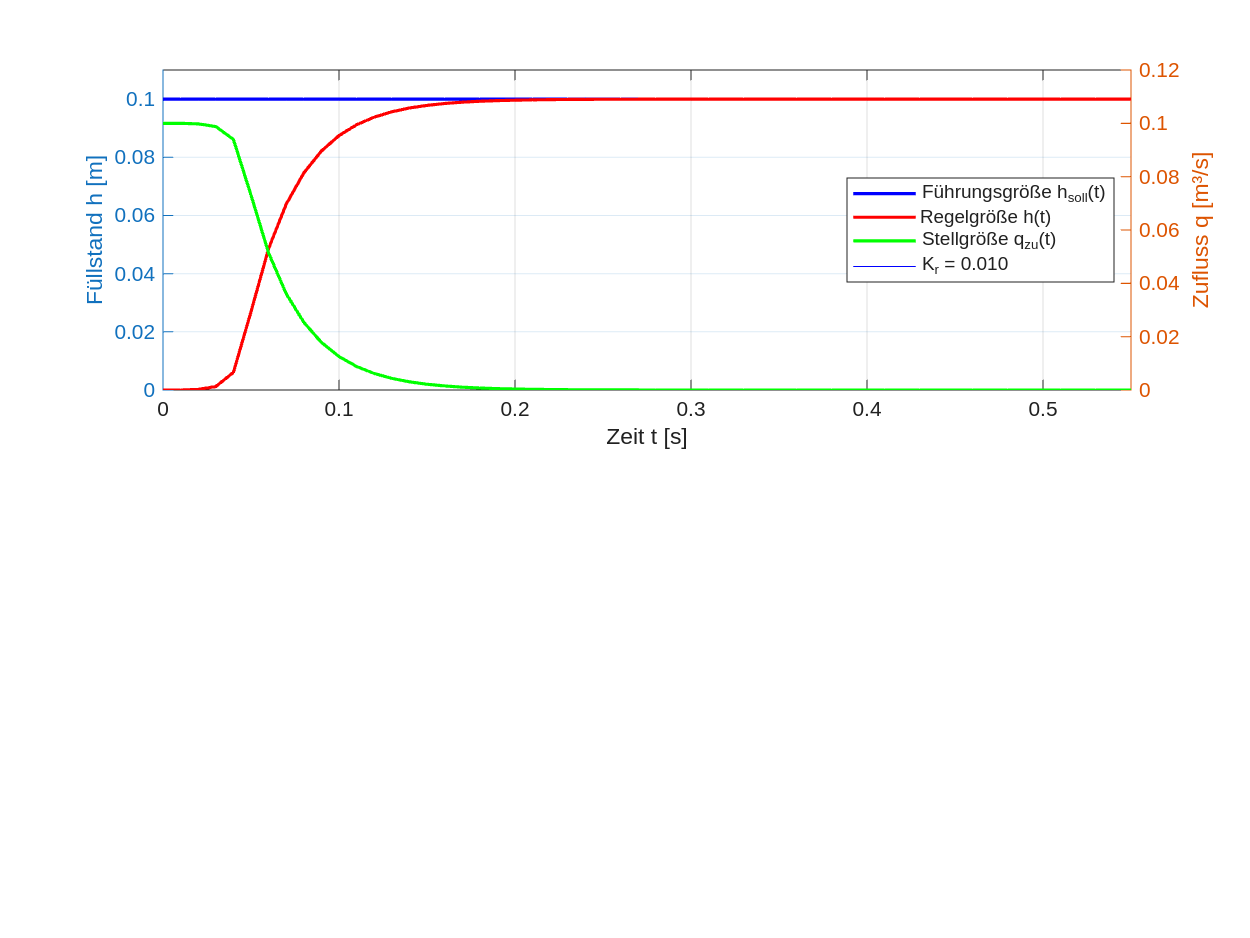
\includegraphics[trim=0cm 8cm 0cm 0.5cm, clip, width=0.9\textwidth]{graphix/modell_ohne_abfluss_KR_0.010.png}
    \end{subfigure}
    
    \begin{subfigure}{\textwidth}
        \centering
        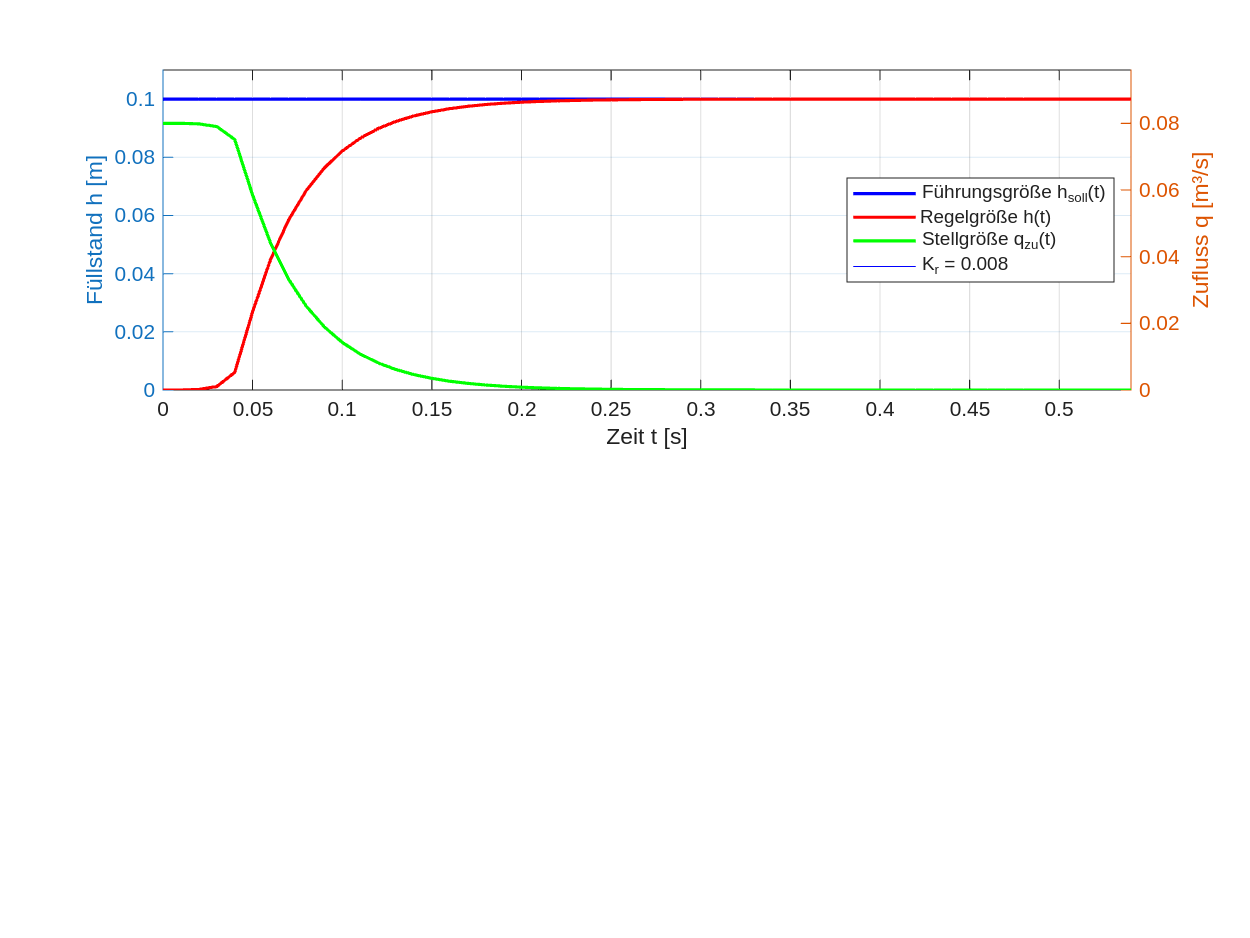
\includegraphics[trim=0cm 8cm 0cm 0.5cm, clip, width=0.9\textwidth]{graphix/modell_ohne_abfluss_KR_0.008.png}
    \end{subfigure}
    
    \begin{subfigure}{\textwidth}
        \centering
        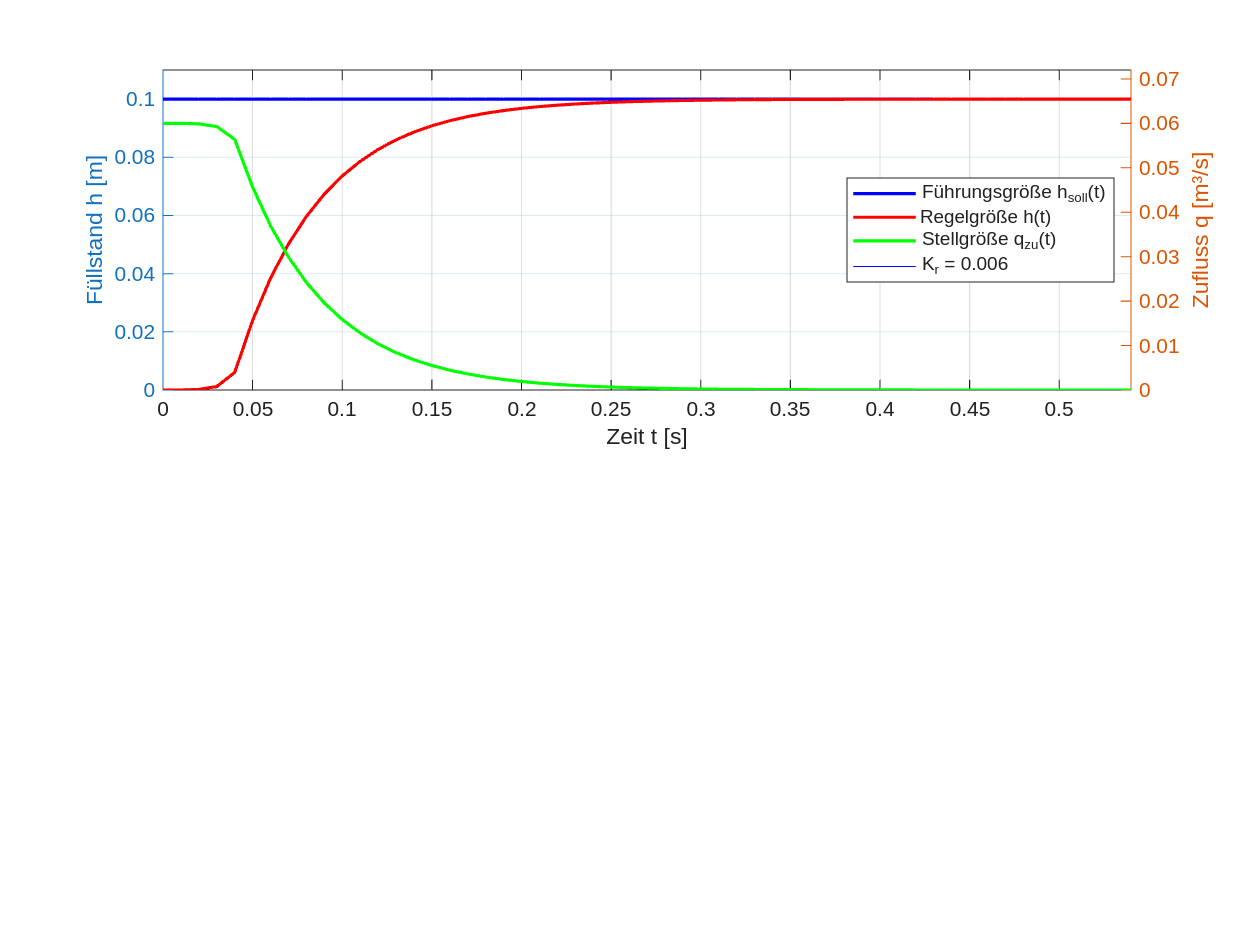
\includegraphics[trim=0cm 8cm 0cm 0.5cm, clip, width=0.9\textwidth]{graphix/modell_ohne_abfluss_KR_0.006.png}
    \end{subfigure}
    
    \begin{subfigure}{\textwidth}
        \centering
        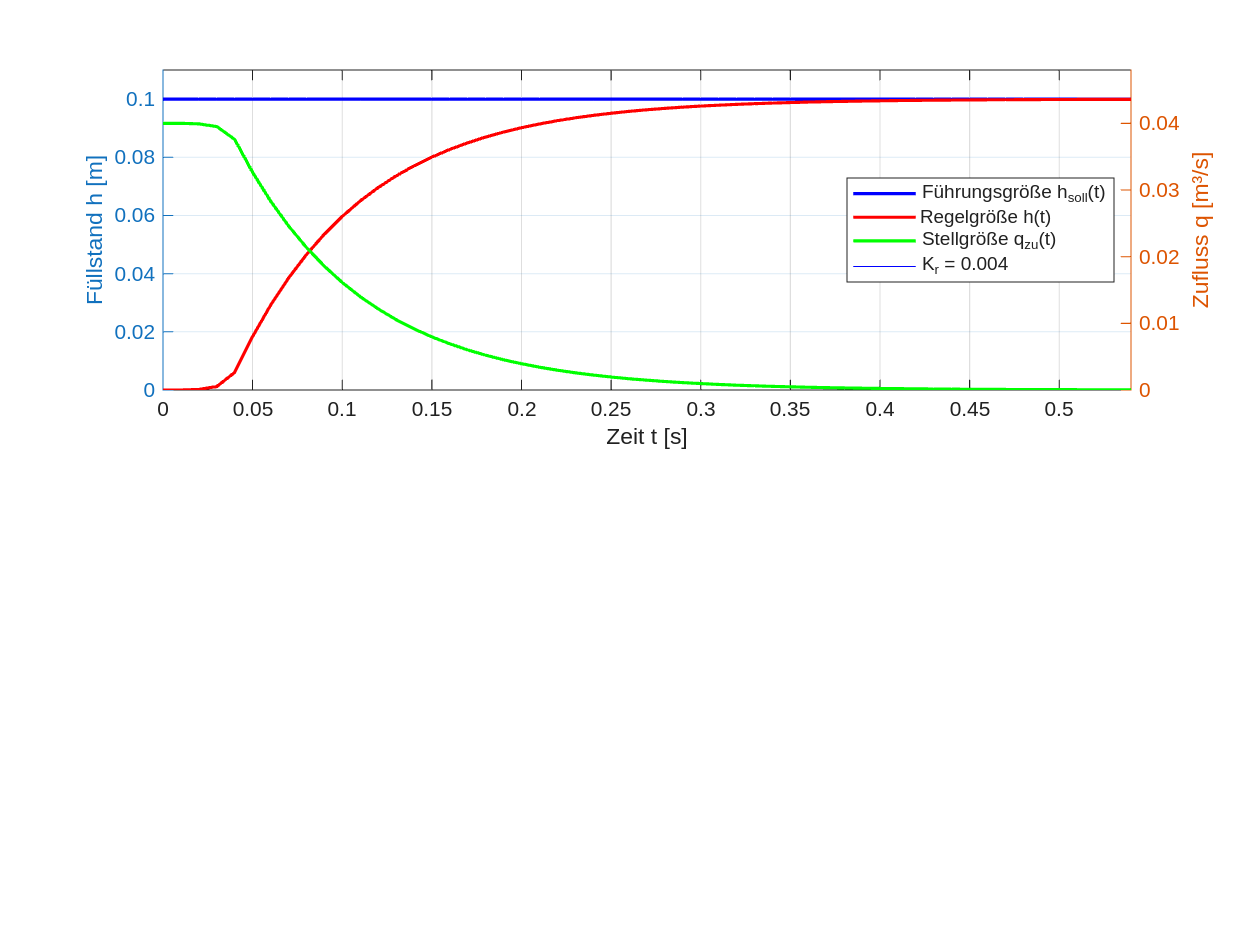
\includegraphics[trim=0cm 8cm 0cm 0.5cm, clip, width=0.9\textwidth]{graphix/modell_ohne_abfluss_KR_0.004.png}
    \end{subfigure}
    
    \begin{subfigure}{\textwidth}
        \centering
        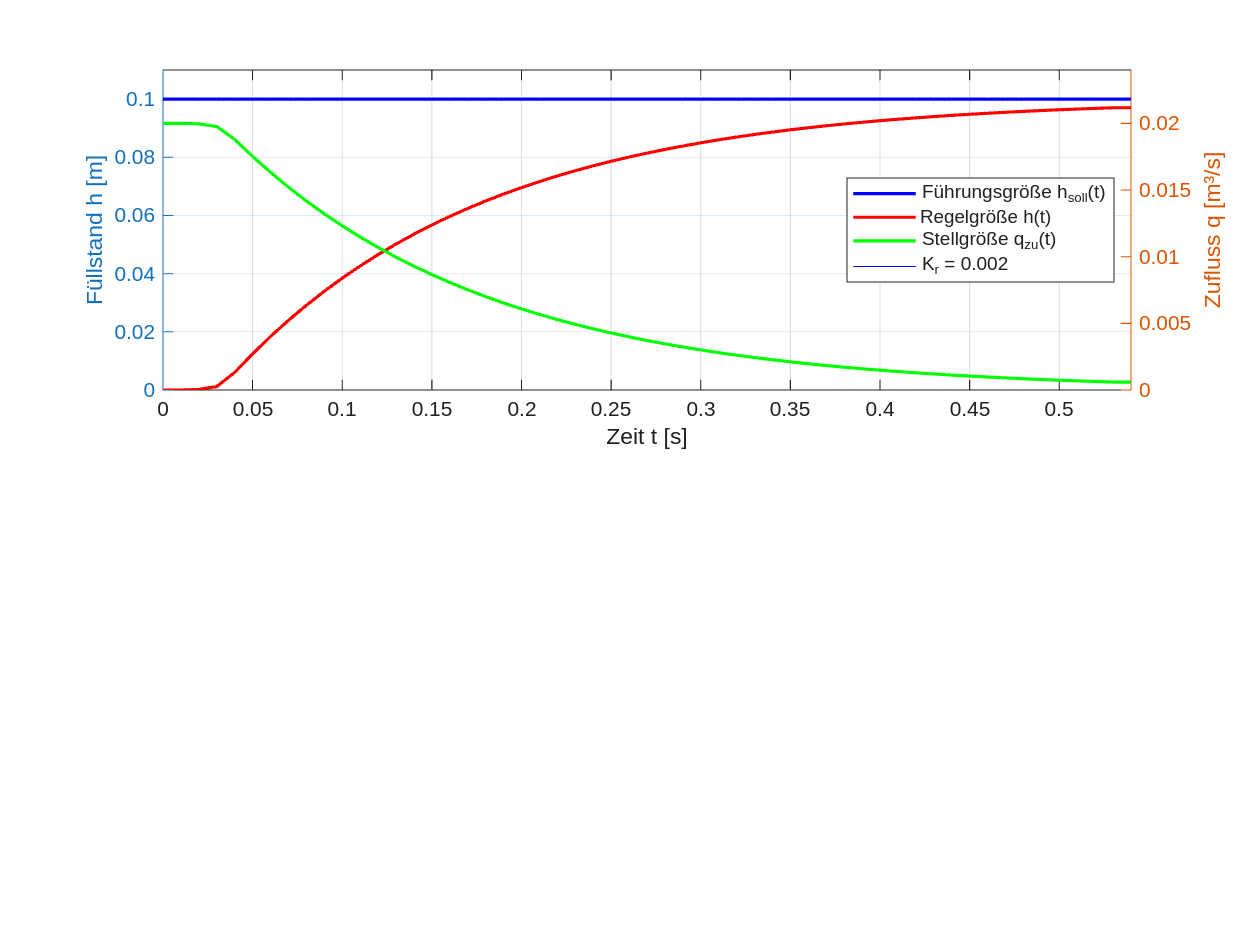
\includegraphics[trim=0cm 8cm 0cm 0.5cm, clip, width=0.9\textwidth]{graphix/modell_ohne_abfluss_KR_0.002.png}
    \end{subfigure}
    
    \caption{\textit{Matlab}-Plots für verschiedene Reglerverstärkungen}
    \label{fig:plots_ohne_abfluss}
\end{figure}




